\graphicspath{{images/}}
\section*{Kontextfreie Grammatiken}

\begin{definition}{Kontextfreie Grammatik} $(K F G)$ ist ein 4-Tupel $(N, \Sigma, P, A)$ mit
    \begin{itemize}
    \item $N$: Alphabet der Nichtterminale (Variablen)
    \item $\Sigma$: Alphabet der Terminale
    \item $P$: endliche Menge von Produktionen mit der Form $X \rightarrow \beta$
    \end{itemize}

    $\quad$ Mit Kopf $X \in N$ und Rumpf $\beta \in(N \cup \Sigma)^{*}$

    \begin{itemize}
    \item $A$: Startsymbol, wobei $A \in N$
    \end{itemize}

    Ein Wort $\beta \in(N \cup \Sigma)^{*}$ nennen wir Satzform.

    Seien $\alpha, \beta$ und $\gamma$ Satzformen und $A \rightarrow \gamma$ eine Produktion.

    \begin{itemize}
    \item Ableitungsschritt mit Produktion $A \rightarrow \gamma \quad \alpha A \beta \rightarrow \alpha \gamma \beta$
    \item Ableitung Folge von Ableitungsschritten $\alpha \rightarrow \cdots \rightarrow \omega$
    \end{itemize}
\end{definition}

\begin{minipage}{0.8\linewidth}
    \begin{definition}{Ableitungsbaum (Parsebaum)} 
        
        KGF für die Sprache $L=\{0^{n} 1^{m} | n, m \in \N\}$
        \begin{itemize}
        \item $G_{1}=\{\{A, B, C\},\{0,1\}, P, A\}$
        \item $P=\{A \rightarrow B C$, $B \rightarrow 0 B$ | $0$ | $\varepsilon$, $C \rightarrow 1 C$ | $1$ | $\varepsilon\}$
        \end{itemize}
        Ableitung von $\omega_{1}=011$:\\ $A \rightarrow B C \rightarrow 0 C \rightarrow 01 C \rightarrow 011$
    \end{definition}
\end{minipage}
\begin{minipage}{0.2\linewidth}
    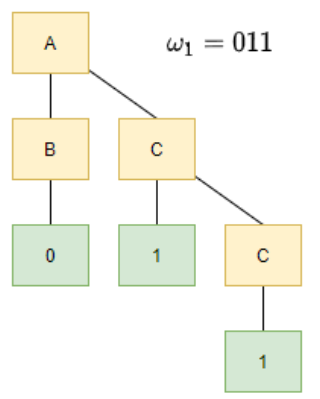
\includegraphics[width=1\linewidth]{images/ableitungsbaum.png}
\end{minipage}





\begin{concept}{Mehrdeutige KFG} $\exists $ Wort, das mehrere Ableitungsbäume besitzt.\\
    Mehrdeutigkeiten eliminieren: Korrekte Klammerung vom Benutzer erzwingen, Grammatik anpassen, Produktionen Vorrang geben
\end{concept}


\begin{KR}{Reguläre Srache durch KFG beschreiben} $\forall$ L $\exists$ KFG

    $L$ reguläre Sprache $\Rightarrow \exists$ DEA $M=\left(Q, \Sigma, \delta, q_{0}, F\right)$ mit $L(M)=L$
    
    \vspace*{1mm}

    KFG für $L$ bauen:
    \begin{itemize}
    \item $\forall$Zustand $q_{i}$ gibt es ein Nichtterminal $Q_{i}$
    \item $\forall$Transition $\delta\left(q_{i}, a\right)=q_{j}$ erstelle Produktion $Q_{i} \rightarrow a Q_{j}$
    \item $\forall$akzeptierenden Zustand $q_{i} \in F$ erstelle Produktion $Q_{i} \rightarrow \varepsilon$
    \item Nichtterminal $Q_{0}$ wird zum Startsymbol $A$.
    \end{itemize}
    ACHTUNG: es dürfen keine Wörter, die nicht in $L$ sind, abgeleitet werden können
\end{KR}

\begin{example2}{KFG für die Sprache} $L=\{0^{n} 1^{n} \mid n \in \N\}$
    
    $G_1 = (\{A\}, \{0,1\}, P, A)$\\
    $P = \{A \rightarrow 0 A 1 | \varepsilon\}$
\end{example2}

\begin{example2}{KFG für die Sprache}$L_5=\{w \in\{0,1\}^* \mid |w|_1 \mod 3=0\}$

    \begin{minipage}{0.6\linewidth}
    Nichtterminale: $Q_0, Q_1, Q_2$

    Produktionen:
    $
    \begin{aligned}
    & Q_0 \rightarrow 0 Q_0 \mid 1 Q_1 \mid \varepsilon \\
    & Q_1 \rightarrow 0 Q_1 \mid 1 Q_2 \\
    & Q_2 \rightarrow 0 Q_2 \mid 1 Q_0
    \end{aligned}
    $
    \end{minipage}
    \begin{minipage}{0.39\linewidth}
        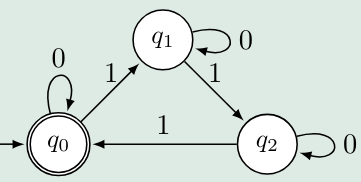
\includegraphics[width=1\linewidth]{images/kfg_reg.png}
    \end{minipage}

    \vspace{1mm}

Beispiel für Ableitung von $w=10011$:
$
Q_0 \Rightarrow 1 Q_1 \Rightarrow 10 Q_1 \Rightarrow 100 Q_1 \Rightarrow 1001 Q_2 \Rightarrow 10011 Q_0 \Rightarrow 10011
$ 
\end{example2}
